\section{Introduction}
Machine learning (ML) has become a significant driving force within the HPC community. New ML algorithms are being developed to analyze the data deluge coming from simulation codes, ``Big Data'' problems, as well as scientific instruments. Unfortunately, I/O bandwidth continues to lag behind compute~\cite{7426274}. However, \textit{in situ} processing~\cite{doi:10.1111/cgf.12930}, which processes the data where it is generated, have stepped in to cope with this I/O bottleneck. These frameworks have become more common in the modern HPC environment. 

Machine learning has a cost, though. Traditionally a researcher develops an algorithm to combine with data to produce a scientific visualization output such as a rendered image or a triangular mesh (Fig.~\ref{fig:ml-vs-trad}). Developing ML algorithms is the inverse of the traditional programming model: data is processed with traditional output (simulation data, high-quality rendered images, etc) to generate ML algorithms. Significant amount of computation as well as copious amounts of traditional output can be required to construct sophisticated ML algorithms. To perform this coupling efficiently at scale, an \textit{in situ} processing is required.

\begin{figure}
    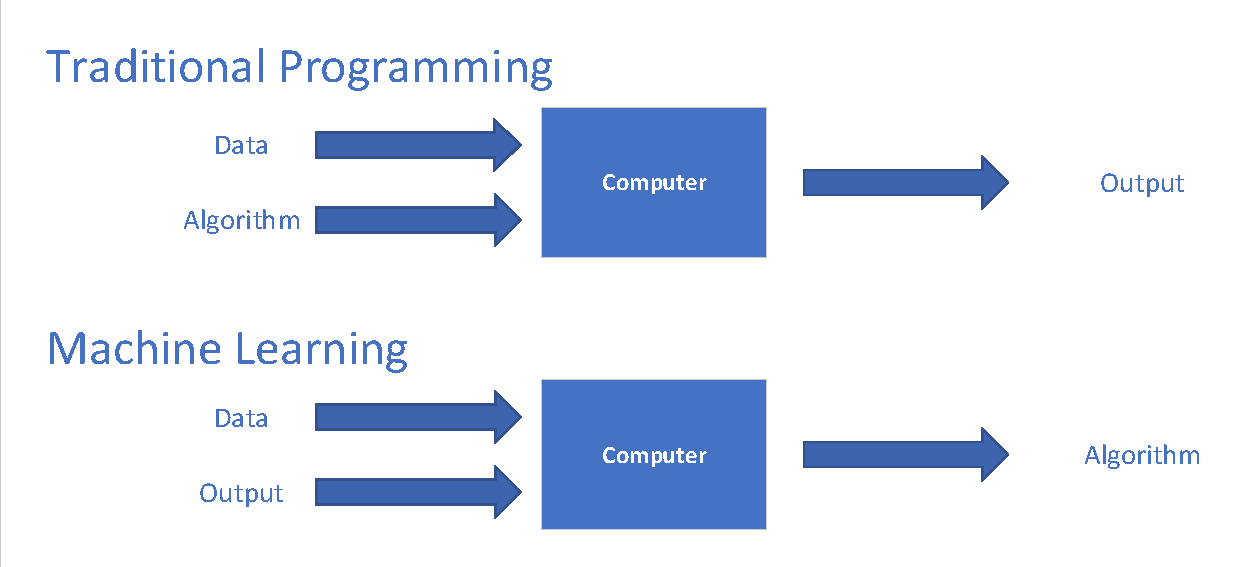
\includegraphics[width=\linewidth]{ML-data-output-program}
    \caption{Traditional programming vs machine learning.}
    \label{fig:ml-vs-trad}
  \end{figure}

In this work we present PAVE, an \textit{in situ} framework for coupling scientific visualization and machine learning. The purpose of this framework is to offer a solution which provides the means necessary to couple machine learning implementations at scale and \textit{in situ} to aid or be the basis of scientific visualisation tasks. We accomplish this by providing read, write and in place data transfer functionality between learning models and visualisation task implementations. To our knowledge, this is the first scientific visualization-machine learning \textit{in situ} framework.

Further, we present a case study of coupling a path-tracer, a physically-based light rendering model, with a neural network to build a filter for a more efficient, but accurate light transport. The case study utilizes VTK-m, a toolkit for massively threaded architectures for scientific visualization and Python, an increasingly popular language within the machine learning community due to robust libraries available for neural networks such as PyTorch. The resulting work accomplishes this combination by utilising VTK-m to construct a path trace rendering tool able to fluidly and efficiently communicate to a cGAN by means of PAVE during training.   The resulting generative model serves as a real-time filter for rendering globally illuminated images which accurately approximate diffuse indirect illumination and soft shadows with quality comparable to offline approaches. 

\begin{figure*}
    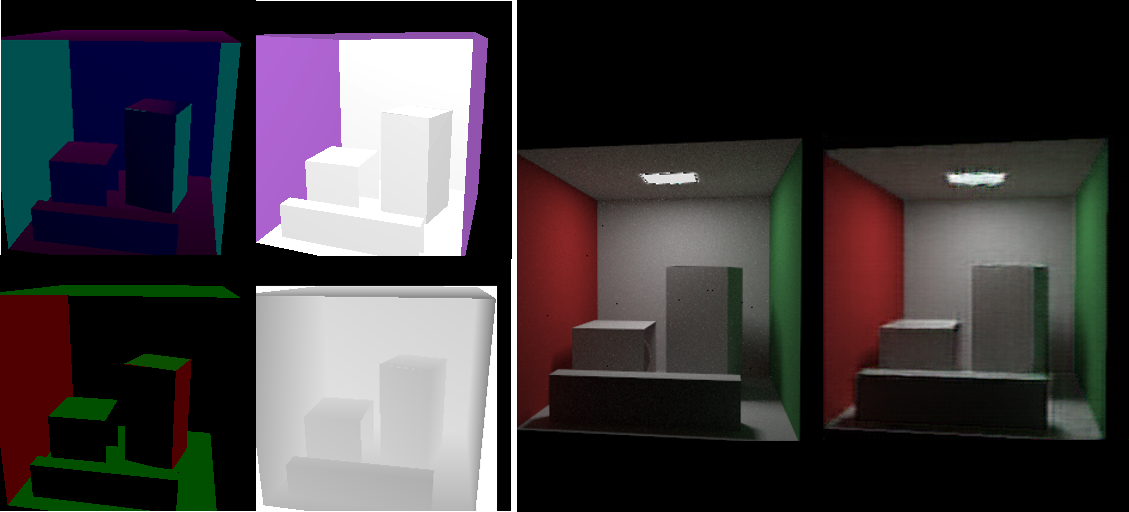
\includegraphics[width=\linewidth]{Teaser.png}
    \caption{Rendered Conditional Geometry Buffers ({\bf left set}) and artificial rendering with conditional generative adversarial neural network ({\bf right couple}) comparing ground truth path traced rendering ({\bf left}) with image generated ({\bf right}).}
    \label{teaser}
  \end{figure*}
